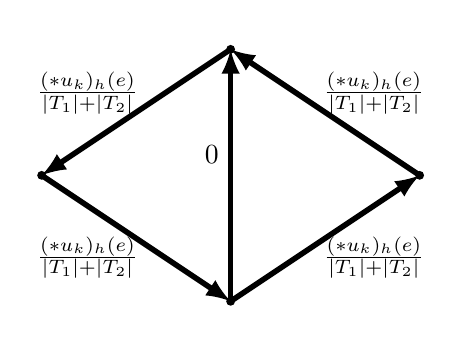
\begin{tikzpicture}[>=latex, line width=2pt, scale=0.8]

%define picture size
\draw[opacity=0] (-3.1,-2.1) rectangle (3.1,2.3);

% vertex coords
\coordinate (V1) at (0,-2);
\coordinate (V2) at (0,2);
\coordinate (V3) at (3,0);
\coordinate (V4) at (-3,0);

%Circumcenters
\coordinate (CC1) at (-0.833,0);
\coordinate (CC2) at (0.833,0);
%\draw[->,gray] (CC2) -- (CC1) node [midway,below right]{$\star e$};

%points
\fill(V1) circle(2pt);
\fill(V2) circle(2pt);
\fill(V3) circle(2pt);
\fill(V4) circle(2pt);

%\fill[gray] (CC1) circle(2pt);
%\fill[gray] (CC2) circle(2pt);

%\node[left] at (CC1) {$T_{1}$};
%\node[right] at (CC2) {$T_{2}$};


%arrows
\draw[->] (V1) -- (V2) node [midway,above left] {$0$} ;
\draw[<-] (V2) -- (V3) node [midway,above right=-5pt] {$\frac{(*u_k)_h(e)}{|T_1|+|T_2|}$};
\draw[->] (V1) -- (V3) node [midway,below right=-5pt] {$\frac{(*u_k)_h(e)}{|T_1|+|T_2|}$};
\draw[<-] (V4) -- (V2) node [midway,above left=-5pt] {$\frac{(*u_k)_h(e)}{|T_1|+|T_2|}$};
\draw[->] (V4) -- (V1) node [midway,below left=-5pt] {$\frac{(*u_k)_h(e)}{|T_1|+|T_2|}$};







\end{tikzpicture}
